%\documentclass[10pt,twocolumn]{article}
\documentclass[10pt]{article}
\usepackage[utf8]{inputenc}
\usepackage[german]{babel}
\usepackage{eurosym}
\usepackage{float}
\usepackage{url}
\usepackage{amsmath}
\usepackage{amsfonts}
\usepackage{amssymb}
\usepackage{graphicx}
\usepackage{paralist}
\usepackage{breqn}
\usepackage{cite}
\usepackage[sort=use]{glossaries-extra}
\usepackage{titlesec}
\usepackage{lipsum}% provides filler text
\usepackage{hyperref}
\usepackage{listings}

\titlespacing{\paragraph}{%
  0pt}{%left margin
  0.1\baselineskip}{% space before (vertical)
  0.1em}%space after (horizontal)
\setlength{\parindent}{0em}
\setlength{\parskip}{1.0em}

% Keywords command
\providecommand{\keywords}[1]
{
  \small	
  \textbf{\textit{Schlüsselwörter --- }} #1
}

\newglossaryentry{api}{name={API},plural={APIs},
description={Die API ist eine Schnittstelle, die ein Softwaresystem bereitstellt, um dieses in andere Programme einzubinden.}}
\newglossaryentry{blockchain}{name={Blockchain},plural={Blockchains},
description={A system in which a record of transactions are maintained across several computers that are linked in a peer-to-peer network.}}
\newglossaryentry{eth}
{name={ETH}, plural={ETH},
description={Standard Währungseinheit im Ethereum Netzwerk.}}
\newglossaryentry{gas}
{name={Gas}, plural={Gas},
description={Gas ist eine Einheit der Rechenarbeit und der Kosten von Transaktionen oder Smart Contracts die im Netzwerk ausgeführt werden.}}
\newglossaryentry{wei}
{name={WEI}, plural={WEI},
description={Kleinste Währungseinheit im Ethereum Netzwerk.}}
\newglossaryentry{GDPR}
{name={GDPR}, plural={GDPR},
description={Die Datenschutz-Grundverordnung ist eine Verordnung der Europäischen Union, mit der die Regeln zur Verarbeitung personenbezogener Daten durch die meisten Datenverarbeiter, sowohl private wie öffentliche, EU-weit vereinheitlicht werden.}}

\begin{document}  
	%\renewcommand{\baselinestretch}{0.4}\normalsize
	
    % NEW SITE ---------------------------------------------------------------------------------

\title{TODO(wieso nur Pension?): DEPOT: A DECENTRALIZED AUTONOMOUS PENSION SYSTEM}
\author{
  Mizel, Paul\\
  \texttt{pmizel@asure.io}\\
  Asure Foundation \\ 
  {\url{https://asure.network}}\\
  \and
  Raetz, Fabian\\
  \texttt{fraetz@asure.io}\\
  Asure Foundation \\ 
  {\url{https://asure.network}}\\
  \and
  Kuchaev, Andrey\\
  \texttt{akuchaev@asure.io}\\
  Asure Foundation \\ 
  {\url{https://asure.network}}\\
}

\date{March 4, 2019\\v1.0}
\maketitle

% \newpage 
% NEW SITE ---------------------------------------------------------------------------------
	\begin{abstract}

Die Asure Stiftung hat sich das Ziel gesetzt, die Sozialversicherungssysteme dieser Welt mit Hilfe der neusten Technologien wie Blockchain zu erforschen und zu verbessern. 
Um die Herausforderungen und die Anforderungen zur Modernisierung und Entwicklung von umlagebasierten Systemen besser verstehen zu können, wurde der Prototyp des deutschen Rentensystems auf der öffentlichen Ethereum Blockchain entwickelt.
In diesem Dokument stellen wir das Ergebnis sowie die im Rahmen der Entwicklung gewonnenen Erkenntnisse vor.

\end{abstract}

\keywords{Blockchain, Ethereum, Sozialversicherung, Rentensystem, Deutsche Rentenversicherung, Umlageverfahren}

	
	\newpage
	%\tableofcontents

    \section{Introduction}

Development over the last 150 years have led to a shift in old-age provision from the family association to larger groups (state, collective of the insured community). Pension systems today are an essential part of the economic development of states and yet, there are 4.1 billion people without access to social security.\cite{noauthor_universal_2017}

There are a variety of pension systems. For instance, in Germany pension systems are categorized into the three pillars of old-age provision. The three pillars include statutory, occupational and private pension systems. Many countries use a similar classification. As a general rule, the more pension systems a person participates in, the better he/she is protected against old-age poverty due to risk diversification.

\paragraph{Financing.} Occupational and private pension systems finance themselves through the funding method and generally follow the performance principle: those who contribute a lot to the pension system also get paid a lot when they get old.

Statutory pension systems finance themselves through the funding method, the pay-as-you-go method or a hybrid of the funding and the pay-as-you-go methods. In addition to the performance principle, many statutory pension insurance policies also follow the principle of solidarity. In Germany, for example, parental leave can be counted as contribution years in pension insurance.

Both the funding method and the pay-as-you-go method have proven their worth in the past. Both financing methods have their strengths and weaknesses, and opinions differ widely as to which financing method is the better one.
%Die Dezentrale Rente soll nach dem Vorbild der %Dezentralisierten Autonomen Organisation (DAO) von der %Community für die Community existieren und mehrere  Probleme %von heute vorhandenen Systeme beheben.

\subsection{Challenges of old-age provision}

Good old-age provision is hard to build. In the following we will discuss some of the challenges of old-age provision and existing pension systems.

\paragraph{Demographic change.} Life expectancy is increasing all over the world, and especially in industrialized nations, the proportion of people over the age of 60 is growing and the problem of retirement provision is becoming more pressing. The burden on pension systems, and in particular PAYG-funded pension schemes, is rising sharply as fewer contributors become available to provide pension payments. The population of developing countries will increase in the future, and thus the problem of retirement provision. For example, the United Nations estimates that by 2050, approximately two billion people will be over 60 years of age, of which as many as 80\% live in developing countries
\cite{noauthor_pensions_2009}.


\paragraph{Inflation.}  In economics, inflation refers to a general and sustained increase in the price level of goods and services (inflation), equivalent to a reduction in the purchasing power of money. The consumer price index (CPR) is most frequently used to measure inflation. The index is calculated with the help of a shopping basket, which is determined in a certain year (base year) representative of an average household. \cite{inflation} 
At an inflation rate of 2\%, this means from \$ 1,000 today, which in 2040 has only a purchasing power of \$ 672.97 in 2040. 
For this reason, it is important not to store the values, but to try to systematically preserve purchasing power by means of a pay-as-you-go system.

\paragraph{Mismanagement and fees.} Compared to pay-as-you-go systems, funded systems are very strongly subject to inflation. For this reason, different investment options are used, these have a higher workload and resulting administrative costs the customer must bear. Another variable is the higher volatility, it increases the chance that the investments are made well as well as the risk that bad investments can be made.

%\paragraph{Entertainment.} Todo:Die jeweils aktive und leistungsfähige Generation betreibt private Altersvorsorge und beteiligt sich zusätzlich ...
%The active and efficient generation in each case operates private old-age provision and also participates ...
%State-organized pension schemes, unlike privately-organized pension schemes, can use both the funded and the pay-as-you-go method.
%The state makes the guarantees and promises to pay out a pension but in the event of a state crisis and a financial collapse even a state will not be able to secure the standard of living, it functions well as long as the economy of a country has a certain stability.

%\paragraph{Funded pension schemes.} Inflation leads to a considerable loss of value in the accumulation of assets as part of old-age provision. 
%Todo: 
%Rentensystem auf Basis des Kapitaldeckungsverfahren investieren Beiträge um eine Rendite zu erzielen, welche den Wertverlust durch die Inflation ausgleicht und im besten Fall zu einer Wertsteigerung führt.

\paragraph{Instrumentalization by politics.} Social security funds are in the hands of politicians and bureaucrats and are perfect for redistributing revenue. This circumstance allows politicians to use social insurance for electoral promises by redistributing them in favor of a group of voters, thus ensuring the next re-election. In addition, governments benefit from more money, power and prestige through social security administration. \cite{zweifel_insurance_2012}

\paragraph{Last generation.} With pay-as-you-go systems, it is important to ensure that there is a next generation, if this is not the case, the last generation will lose the most in the system as nobody is left to pay their pensions.

\paragraph{Residual risk.} 
We do not want to go into detail about other risks such as economic risk, credit risk, interest rate risk, volatility, currency risk, psychological market risk, liquidity risk, tax risks, information risk, country and transfer risk.
All pension systems are not risk-free, this is in the nature of risk-oriented systems, the solutions are based on risk minimization, through various approaches such as risk diversification, risk taking by the country, alternative pensions such as real estate and passive income, a pension plan can be well implemented.


\subsection{Our approach: Decentralized pension}
The invention of the Ethereum blockchain with its build-in Turing complete programming language, made it possible to write smart contracts and decentralized applications that create their own arbitrary rules of ownership, transaction formats and state transition functions. \cite{buterin2013whitepaper} Since Ethereum, many more blockchains (\cite{hyperledger}, \cite{stellar} ,\cite{cordano}) with build-in Turing complete programming languages and different trade-offs are available.

Our approach of a decentralized pension is to provide a state transition function of a \textbf{pay-as-you-go} financed pension system as a smart contract and therefore inherit many exiting properties of the underlying blockchain-technology.

Through our \textbf{preliminary work} and engagement with pension systems, we've created the \textbf{requirements} to a decentralized pension model that define \textbf{target audience} and use the \textbf{pay-as-you-go} basis and the \textbf{ incentivation} methods and the resulting \textbf{benefits} are described in this chapter.

\subsubsection{Requirements}
We talked to experts from insurance and pension systems to develop a model that works decentrally.

Since geopolitical reasons make it impossible for us to attach importance to these conditions, we have developed alternative solutions.
We create incentives in order to help people to pay contributions. With the contribution value we lead a reference contribution rate representative of members which dynamically adapts to the behaviour of the members.

The most important requirement was to enable the storage of purchasing power. Another important factor is to make risk sharing in the community as fair as possible for the target groups for whom it is suitable.

\subsubsection{Target group}
The target groups for a decentralized pension system are people:

\begin{compactitem}
\item without pension access
\item where there is a pension, but
 \begin{compactitem}
 \item it is corrupt
 \item it is intransparent
 \item the country suffers from high inflation
 \item too high administrative costs
 \item no good investment strategies in the pension system
 \item less trust in the government, politics and pension system
 \end{compactitem}
\item which as a further supplement 
 \begin{compactitem}
 \item first mover, technology lover
 \item spread their risks over several risk classes
 \item want to use a decentralized pension solutions
 \item who live as a digital nomad
 \item looking for alternatives
 \end{compactitem}
\end{compactitem}

\subsubsection{Pay-as-you-go system}


Pay-as-you-go systems have great advantages in that they can be introduced quickly and no capital needs to be built up.

The goal of pay-as-you-go is to store the purchasing power of the system in the economic sense, to the pension points per deposit are stored as a representation of the contribution and not the contribution value.
At retirement, the pension contribution is calculated on the basis of these points at the reference value\footnote{Example: In germany, it is linked to 18.6\% of the salary in 2019.}.


\subsubsection{Incentives}
Decentralized solutions such as decentralized pensions can only grow organically over the years thanks to a well thought-out incentive structure. Since the use is left to a user, it is comparable with Bitcoin\cite{nakamoto2012bitcoin}, as the system is only controlled by trust and incentives.
%TODO:dass sich dieses System nur durch Vertrauen und die Anreize.

\subsection{Our contribution}
As an inspiration we have oriented ourselves on the German pay-as-you-go system. After having implemented the German pension system on Ethereum in outline, we have seen the challenges that needed to be solved.

In addition to the challenges, we also saw opportunities to improve the system, such as the degree of automation and the creation of new incentives that are not dependent on middlemen.

There are many advantages that a decentralized pension system can offer, the most important of which we will discuss here.

\paragraph{Decentralized and Autonomous.} With the help of blockchain technology, the system is available decentralized and this allows 24/7 access worldwide. There are no employees required to operate the system and this reduces administration costs enormously.

\paragraph{Reduces costs.} Due to the automation and decentralized operation, there is no additional cost apart from the transaction fees \footnote{Except for the Tx fees, these charges may differ depending on the network used, such as Ethereum.}.

\paragraph{Transparent.} It is open-source and anyone can view the transactions and check the validity of the processes in the system.

\paragraph{Permissionless.} 
Access is available to everyone and worldwide unconditionally. Access to this system is available to anyone with Internet access.

\paragraph{Without any intermediaries.} 
There is no organization or middleman who have money access, the system is a closed economy in itself.


\paragraph{Corruption free.} There's no way we can steal the money.

\paragraph{Tamper-proof.} The permitted changes of the system are left to the members.

\paragraph{Fraud free.}
Fraud is avoided by the fact that we do not need external information for the operation. 

\paragraph{100 years life cycle.} 
The system is designed to last 100 years, with a 20-year system start and a 40-year payment period \footnote{ Different products with different running times can be created.}.  

\paragraph{Base points limit to 2.0 points.} 
Pension points are limited on the basis to 2.0, this has the background that no one may have an incalculable claim in the later redistribution.

\paragraph{Fully inheritable.}
The total pension entitlement can be inherited by passing on the private key.

\paragraph{GDPR compliant\cite{gdpr}.} 
We do not use any external data sources such as age, death certificate and average salary as reference values.

\paragraph{Incentive system.} 
Several incentives ensure the sustainability and adoption of the system in the community.



	\section{Implementierung}
Im folgenden Kapitel betrachten wir die Implementierung des Prototypen.


\subsection{OpenSource}
Der Quellcode des entwickelten Prototypen ist auf GitHub\footnote{\url{https://github.com/AsureNetwork/asure-dapp}} veröffentlicht und kann unter der ISC Lizenz\footnote{\url{https://github.com/AsureNetwork/asure-dapp/blob/master/LICENSE}} im Rahmen weiterer Softwareprojekte genutzt werden.

\paragraph*{}
Der Prototyp steht unter der Adresse \url{https://dapp.asure.io/} zum testen bereit. 

\subsection{Anwendungsfälle}
Das deutsche gesetzliche Rentensystem basiert im Kern auf der Rentenformel, durch welche die Höhe der Rentenzahlung jedes Rentenempfänger ermittelt wird. Durch eine Vielzahl von Sonderregelungen gestaltet sich das Rentensystem jedoch sehr komplex, weshalb eine vollumfängliche Abbildung des Systems im Rahmen eines Prototypen nicht sinnvoll ist. Stattdessen wurden einige Anwendungsfälle ausgewählt, und im Umfang an die Anforderungen eines Prototypen angepasst.

\paragraph{}
Alle Anwendungsfälle zusammen, bilder den kompletten Zyklus eines Rentensystems ab - Von der Zahlung der Beiträge, bis zur Zahlung der Renten.

\paragraph{}
Die Anwendungsfälle sind wie folgt definiert:

\begin{compactenum}
\item Als Benutzer möchte ich mich als Versicherter registrieren.
\item Als Beitragszahler möchte ich mein geplantes Renteneintrittsdatum festlegen.
\item Als Beitragszahler möchte ich jeden Monat in das Rentensystem einzahlen.
\item Als Rentner möchte ich jeden Monat eine Rente auszahlen.
\item Als Versicherter möchte ich eine Übersicht über meine Beiträge / Rentenzahlungen angezeigt bekommen.
\item Als Versicherter möchte ich alle Aktionen via Smartphone Anwendung durchführen.
\item Als Administrator möchte ich das Backend (Smart Contracts) auf dem öffentlichen Ethereum Testnet bereitstellen.
\end{compactenum}


\subsection{Deutsche Rentenformel}
Für die Berechnung der Höhe der Renten wurde die deutsche Rentenformel (Siehe \ref{eq:rentenformel}) verwendet.
\\
Dabei wurde im Rahmen des Prototypen nur die Berechnung der Entgeltpunkte (EP) implementiert. 
\\
Der Wert für den Zugangsfaktor (ZF) als auch für den Rentenartfaktor (RAF) ist immer 1. Hieraus resultiert, das die berechneten Renten immer einer Rente wegen Alters und regulären Rentenbeginn entsprechen.
\\
Auch der Wert für den aktuelle Rentenwert (aRW) ist statisch und beträgt immer \EUR{29}. Der entsprechende Quellcode für die Ermittlung des aktuellen Rentenwerts (aRW) ist so strukturiert, das dieser pro Jahr im System mittels einer Lookup Tabelle hinterlegt werden kann.

\begin{equation*} \label{eq:rentenformel}
Rente_{mtl} = EP \cdot ZF \cdot RAF \cdot aRW
\end{equation*}

\begin{compactitem}
\item \textbf{Rente\textsubscript{mtl}} ist die monatliche Bruttorente in Euro
\item \textbf{EP} ist die Summe der Entgeltpunkte aufgrund des Versicherungsverlaufs
\item \textbf{ZF} ist der Zugangsfaktor
\item \textbf{RAF} ist der Rentenartfaktor
\item \textbf{aRW} ist der aktuelle Rentenwert in Euro
\end{compactitem}


\subsection{Anwendungsarchitektur}
Die Benutzeroberfläche des Prototypen wurde als Progressive Web App (PWA) entwickelt und für die Verwendung auf Mobilgeräten optimiert. Ein Webserver liefert die Webanwendung mittels HTTP/HTTPS an den Browser.
\\
Das Backend bildet ein Smart Contract-System, welches auf dem öffentlichen Ethereum Testnetz Rinkeby gehostet wird und mit dem die Benutzeroberfläche mittels HTTP/WebSockets kommuniziert. Für den Zugriff auf ein Ethereum Netz wird ein Ethereum Knoten (ggf. auch ein Ethereum Cluster für Ausfallsicherheit) benötigt. Im Rahmen des Prototypen verwenden wir hierzu Hosting Provider wie Infura und Cloudflare, welche entsprechende Ethereum Knoten hosten und zur Verfügung stellen.

\begin{figure}
    \centering
    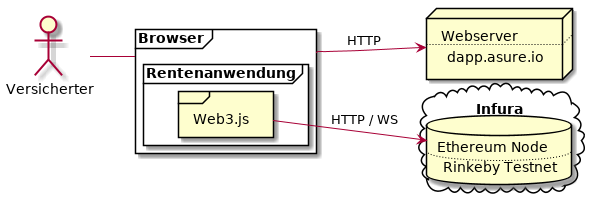
\includegraphics[width=6.0in]{images/components.png}
    \caption{Komponenten des Prototyps}
\end{figure}


\subsection*{Smart Contract Entwicklungswerkzeuge}
Im Rahmen der Backend Entwicklung wurde ein Smart Contract System für die Ethereum Blockchain entwickelt. Für die Entwicklung kamen die folgenden Tools zum Einsatz:

\paragraph*{Solidity} ist eine objektorientierte, anwendungsspezifische höhere Programmiersprache mit einer JavaScript-ähnlichen Syntax zum Entwickeln von Smart Contracts für Blockchain-Plattformen wie Ethereum oder Tron.\\ %TODO cite
Sämtliche Smart Contracts des Prototypen wurden in Solidity programmiert.

\paragraph*{OpenZeppelin Contracts} ist ein Framework aus modularen, wiederverwendbaren und sicheren Smart Contracts für das Ethereum-Netzwerk, geschrieben in Solidity.

\paragraph*{Truffle} ist ein Entwicklungsframework für Ethereum. Es bietet u.a. Funktionen für das Erstellen von automatisierten Tests, Deployment und Migration von Smart Contracts und das Verwalten von verschiedenen Ethereum Netzen wie z.B. ein lokales Entwicklungsnetz, oder das öffentliche Ethereum Testnetz Rinkeby.

\paragraph*{Ganache} ist eine Ethereum Software, welche speziell für die Entwicklung von Smart Contracts entwickelt wurde. Ganache bietet Erweiterungen um z.B. innerhalb von Unit Tests die Uhrzeit zu Manipulieren und somit auch Uhrzeitabhängige Funktionalitäten zu testen.

\paragraph*{Infura} bietet einen skalierbaren API-Zugriff auf öffentliche Ethereum-Netzwerke.


\subsection{Smart Contract Architektur}

\begin{figure}[H]
    \centering
    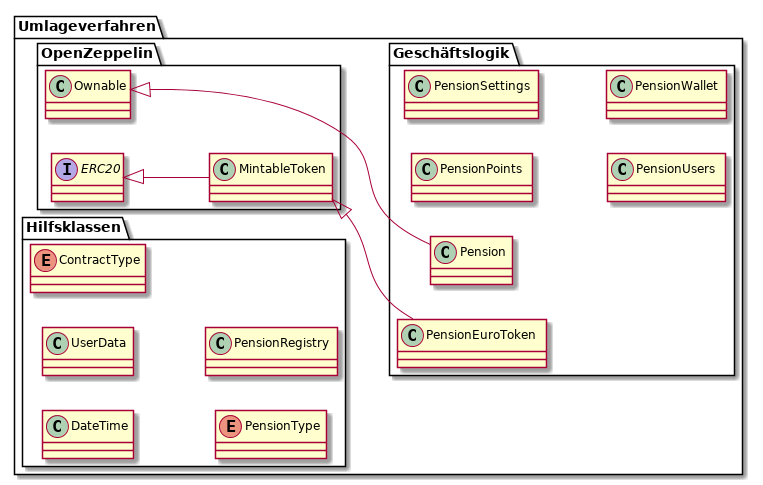
\includegraphics[width=6.0in]{images/classdiagram-smartcontracts.png}
    \caption{Smart Contracts Übersicht}
    \label{fig:asure_architecture}
\end{figure}


\paragraph*{PensionUsers:} Registrierung und Verwaltung von Benutzern und deren Stammdaten.

\paragraph*{PensionWallet:} Beitrags-, und Rentenzahlungen - Verwaltet sämtliche Geldmittel.


\paragraph*{PensionPoints:} Datenhaltung Beitragszahlungen und Entgeltpunkte.

\paragraph*{Pension:} Berechnung der Höhe der Rentenzahlungen.

\paragraph*{PensionSettings:} Verwaltung diverser Parameter (z.B. Rentenartfaktor (RAF) / Rentenwerte (aRW)).

\subsubsection{Anwendungsfall: Als Beitragszahler möchte ich jeden Monat in das Rentensystem einzahlen}

\begin{figure}[H]
    \centering
    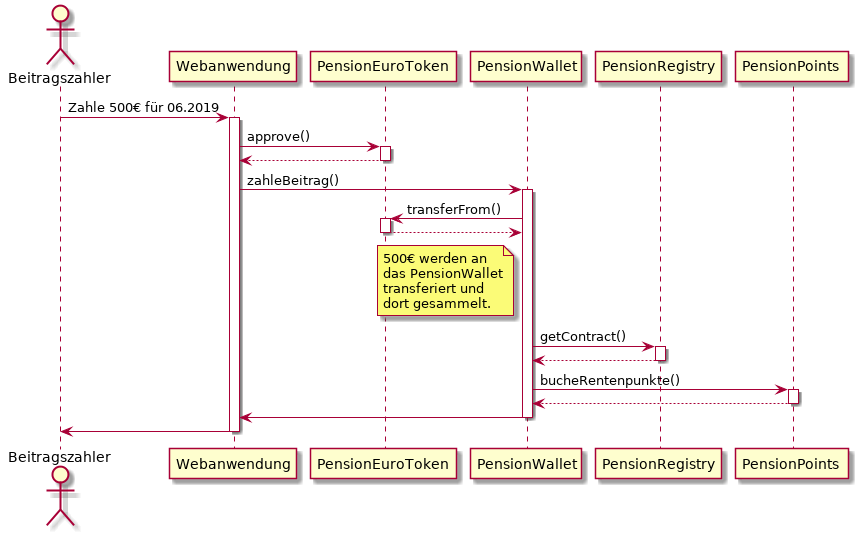
\includegraphics[width=6.0in]{images/usecase-pay.png}
    \caption{Sequenzdiagram: Beitragszahlung}
    \label{fig:asure_architecture}
\end{figure}

\subsubsection{Anwendungsfall: Als Rentner möchte ich jeden Monat eine Rente auszahlen}

\begin{figure}[H]
    \centering
    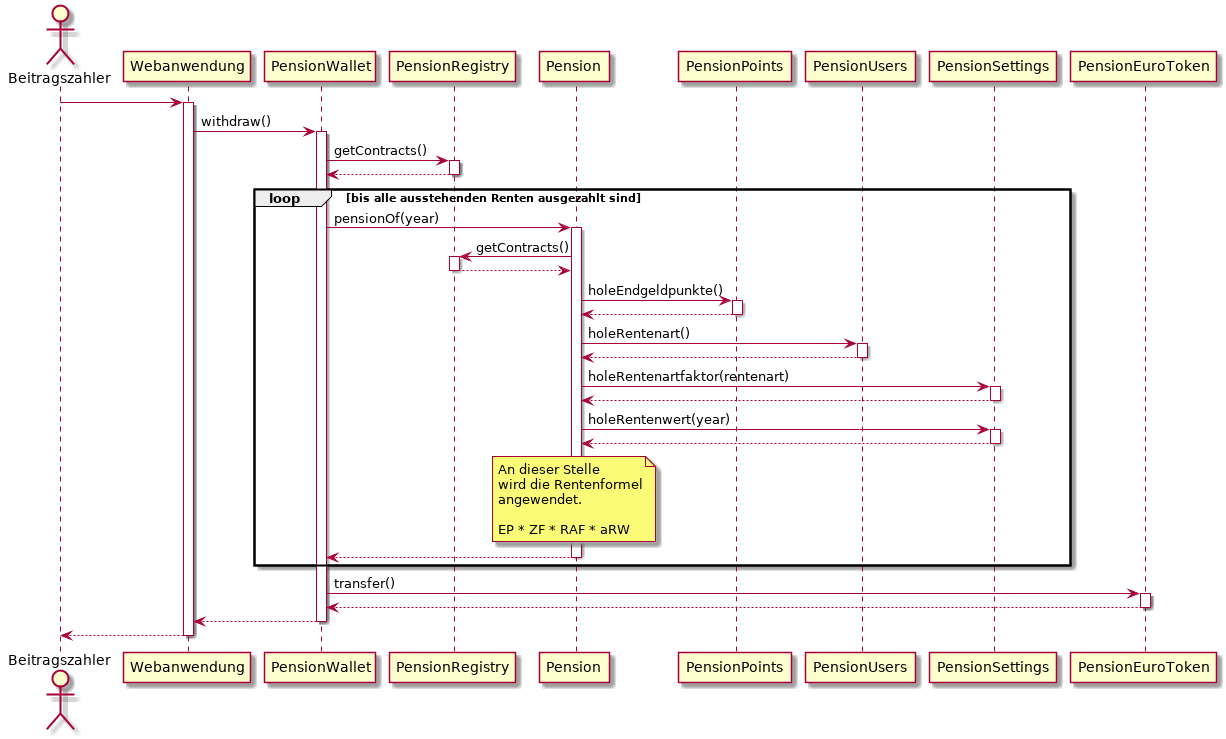
\includegraphics[width=6.0in]{images/usecase-payout.png}
    \caption{Sequenzdiagram: Rentenzahlung}
    \label{fig:asure_architecture}
\end{figure}
	\section{Gewonnenen Erkenntnisse}


\subsection{Mathematische Operationen mittels SafeMath}
Arithmetische Operationen in Solidity werden bei einem Überlauf und Unterlauf umgebrochen. Dies kann leicht zu Fehlern führen, da Programmierer normalerweise davon ausgehen, dass ein Überlauf einen Fehler auslöst, was das Standardverhalten in höheren Programmiersprachen ist.

Das folgende Listing \ref{lst:mul} demonstriert das Problem des Überlauf und Unterlauf einer Integer Variable.

\begin{lstlisting}[caption={Beispielhafter Überlauf und Unterlauf},captionpos=b,label=lst:mul]
contract Test {
  function overflow() returns (uint8) {
    uint8 a = 255;
    a = a + 1;  	
    return a; // a = 0
  }
  
  function underflow() returns (uint8) {
    uint8 a = 0;
    a = a - 1;  	
    return a; // a = 255
  }
}
\end{lstlisting}

\subsubsection*{Lösungsansatz}
Durch das explizite prüfen können Überlaufe und Unterläufe erkannt werden und die Transaktion zurückgesetzt werden. Das OpenZeppelin-Framework stellt eine solche Prüfung mittels der SafeMath API zur Verfügung. SafeMath stellt diese Intuition wieder her, indem die Transaktion zurückgesetzt wird, wenn ein Vorgang überläuft. \cite{safemath}

\begin{lstlisting}[caption={Beispielhafte Multiplikation mittels SafeMath zurück},captionpos=b,label=lst:mulsafe]
contract Test {
 using SafeMath for uint8;

 function multiplySafe(uint8 a) returns (uint8) {
   return a.mul(a); // revert() transaction on overflow / underflow
 }
}
\end{lstlisting}


\subsection{Gleitkommaoperationen}
Die Programiersprache Solidity unterstützt Gleitkommaoperationen nach IEEE 754 nicht. Es gibt jedoch teilunterstützung für Bruchwerte die bestimmten Einschränkungen unterworfen sind.\cite{fixedpointnumbers}

\subsubsection*{Lösungsansätze}

\paragraph*{}
Anstelle von Gleitkommaoperationen, können alternativ entsprechend große Ganzzahlen verwendet werden. Als Beispiel dient z.B. die native Kryptowährung ETH der Ethereum Blockchain. Ein ETH ist eine 19-stellige Ganzzahl. Die kleinste Einheit ist 1 WEI. Ein ETH ist gleich 1.000.000.000.000.000.000 WEI. Durch diese Darstellung können auch Bruchteile eines ETH transferiert werden.

Der Rentenartfaktor (RAF) der Rentenformel ist als Gleitkommazahl definiert und kann Werte von 0 bis 1 annehmen. \cite{raf}

Gleitkommazahlen können auch in diesem Fall durch entsprechend große Ganzzahlen repräsentiert werden, indem im SmartContract immer mit dem Faktor 1000 multipliziert wird. Externe Systeme wie z.B. eine Webanwendung können die Höhe der monatlichen Rente errechnen, indem der Wert entsprechend durch den Devisor 1000 geteilt wird.

\begin{lstlisting}[caption={Verzicht von Gleitkommazahlen durch Multiplikation},captionpos=b,label=lst:simfloat]
contract Rentenformel {
 function rechneBeispiel() returns (uint256) {
   uint256 ep = 40;
   uint256 zf = 1;
   uint256 raf = 250; // kleine Witwenrente = 0.25 * 1000
   uint256 arw = 30;
   
   uint256 mtlRente = ep * zf * raf * arw; // mtlRente = 300000;
   
   return mtlRente; 
   // Extern z.B. in Webanwendung: mtlRente / 1000 = 300
 }
}
\end{lstlisting}

\paragraph*{}
Alternativ kann auf Bibliotheken wie z.B. DS-Math \footnote{\url{https://github.com/dapphub/ds-math}} zurückgegriffen werden, welche entsprechende Funktionalitäten bieten


\subsection{Zeitkomplexität von Smart Contract Methoden}

Jede Ethereum-Transaktion (somit auch jede Ausführung einer Smart Contract Methode) verbraucht "Gas". Pro Transaktion steht nur eine bestimmte Menge an Gas zur Verfügung. Somit sind die Ausführungszeiten und die Aufgaben, welche inerhalb einer Smart Contract Methode ausgeführt werden können, ebenfalls begrenzt. 
Verbraucht eine Ethereum-Transaktion zu viel Gas, wird die Transaktion abgewiesen und nicht in die Blockchain mit aufgenommen.

\subsubsection*{Lösungsansatz}
Die Zeitkomplexität\footnote{\url{http://www.inf.fu-berlin.de/lehre/SS12/ALP2/slides/V6_Rekursion_vs_Iteration_ALP2.pdf}} von SmartContract Methoden sollte immer konstant sein (O(1)). Zeitkomplexität kann reduziert werden, in dem Daten vorberechnet und aggregiert werden.

\paragraph*{} 
Statt wie in Listing \ref{lst:complexitybad} über eine Liste aller Beitragszahlungen zu iterieren, kann die Gesamtsumme aller Beitragszahlungen schon in zahleBeitrag aggregiert werden, sodass die Zeitkomplexität immer O(1) ist.

\begin{lstlisting}[caption={Schlecht - Zeitkomplexität von summeBeitragszahlungen() ist O(n)},captionpos=b,label=lst:complexitybad]
contract Rente {
 uint256[] beitragszahlungen;

 function zahleBeitrag(uint256 beitrag) public {
	beitragszahlungen.push(beitrag);
 }
 
 function summeBeitragszahlungen() public returns (uint256) {
	uint256 summe = 0;
	for (var i = 0; i < beitragszahlungen.length; i++) {
      summe += beitragszahlungen[i];
	}
	return summe;	
 }
}
\end{lstlisting}


\begin{lstlisting}[caption={Gut - Zeitkomplexität von summeBeitragszahlungen() ist O(1)},captionpos=b,label=lst:complexitygood]
contract Rente {
 uint256[] beitragszahlungen;
 uint256 summe;

 function zahleBeitrag(uint256 beitrag) public {
	beitragszahlungen.push(beitrag);
	summe += beitrag;
 }
 
 function summeBeitragszahlungen() public returns (uint256) {
	return summe;	
 }
}
\end{lstlisting}


\subsection{Weitere Beschränkungen bzgl. Smart Contract Programmierung}

\paragraph*{}
Solidity unterstüzt nur statische Zeichenketten. Dynamische Operationen wie das Zusammensetzen von Zeichenketten ist somit ohne weiteres nicht möglich.

\paragraph*{}
Die größe von Smart Contract Quellcode, welche mit einer Transaktion veröffentlicht werden kann, ist beschränkt. Ggf. müssen Zusammenhängende Smart Contract Systeme auf mehrerer Transaktionen aufgeteilt und veröffentlicht werden.

\paragraph*{}
Das Hinterlegen von Smart Contract Quellcode in  Blockchain Explorer (Etherscan.io) ist noch nicht in Truffle integriert und muss händisch durchgeführt werden.


\subsection*{Codeänderungen (Bugfixes und Features)}
Bereitgestellter Smart Contracts Code ist unveränderbar auf der Blockchain gespeichert
Änderungen müssen im Zuge von Fehlerbehebungen und Anforderungsänderungen durchgeführt werden können.

\subsubsection*{Lösungsansatz: Upgradeability Proxy Muster}

\begin{figure}[H]
    \centering
    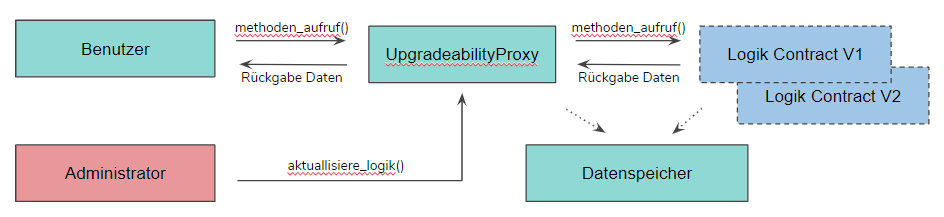
\includegraphics[width=6.0in]{images/pattern-upgrade.png}
    \caption{Smart Contract Upgrade Pattern}
    \label{fig:asure_architecture}
\end{figure}

\subsection*{Abfragen von Blockchain Daten}
Ethereum Smart Contracts bieten nur eine primitive Datenhaltung und rudimentäre Datenabfrage durch Drittanwendungen. 
Benutzer Masken benötigen viele HTTP-Anfragen um die benötigten Daten aus Ethereum in die Anwendung zu laden.

\subsubsection*{Lösungsansatz}
Trennung von Lese-, und Schreiboperationen (Siehe z.B.: CQRS Entwurfsmuster). Spezialisierte Abfrage Proxies z.B. mittels GraphQL (Siehe EthQL und TheGraph)


\subsection*{Batch-Job Verarbeitung}
Ethereum bietet keine native Unterstützung für “zeitgesteuerte” Transaktionen.
Ethereum Smart Contracts können nicht direkt auf Smart Contract Ereignisse reagieren

\subsubsection*{Lösungsansatz}
Externe Systeme können zeitgesteuert und auf Smart Contract Events reagieren - Die Lösung setzt voraus, dass einem externen System “vertraut” wird.


\subsection*{Anbindung externer Datenquellen}
Smart Contracts können nicht auf externe Daten zugreifen (z.B. mittels HTTP)

Als Lösung bieten sich Orakel (Oracles) an. Diese stellen die Daten auf der Blockchain zur Verfügung und stellen auf Anfrage weitere bereit.

Es gibt Oracle-Anbieter, welche die notwendige Infrastruktur bereitstellen und als Dienstleistung genutzt werden können.

Oracle Anbieter: Oraclize, Chainlink, Provable

Entwicklung Projektbezogener Oracles ist eine weitere Option


\subsection*{Transaktionszeiten und Ladeanimationen}
Transaktionen im Ethereum Rinkeby Netzwerk dauer ca. 15 Sekunden. 
Ladeanimationen wie bei klassischen Webanwendungen (1-3 Sekunden) daher schwierig


\subsection*{Wallet Integration}
Wallet Connect
	\section{Fazit}
Im Rahmen dieses Projektes wurde ein Prototyp zum deutschen Rentensystem auf der öffentlichen Ethereum Blockchain entwickelt. Der Prototyp ist im Funktionsumfang stark reduziert und implementiert die Berechnung der Entgeltpunkte (Faktor EP der Rentenformel) als Smart Contract System. Der Zugriff auf das Smart Contract System erfolgt durch eine mobile Webanwendung. Durch diese können Rentenbeiträge mittels der Kryptowährung ETH gezahlt, Renten ausgezahlt und allgemeine Parameter wie z.B. der Zeitpunkt des Renteneintritts spezifiziert werden.

Diese Machbarkeitsstudie des Umlageverfahrens der deutschen Rente auf Ethereum Blockchain hat aufgezeigt, dass der Durchsatz von 7-15 Transaktionen pro Sekunde in Kombination mit anderen Anwendungsfällen für ein Rentensystem in Deutschland nicht ausreicht. Bei Erweiterungen und vollständiger Umsetzung aller Anforderungen, wäre das öffentliche Ethereum Netzwerk heute nicht in der Lage die Verarbeitung ohne großen Aufwand zu unterstützen.

Die Blockchain-Technologie ist Stand 2019 noch in diversen Bereichen limitiert. Es gilt, die Stärken der Blockchain im Kontext von Sozialversicherungen sinnvoll zu nutzen, sodass diese die Schwächen überwiegen. Grundlegende Probleme wie die Skalierung oder der richtige Umgang mit personenbezogenen Daten werden durch diverse Projekte und Institutionen erarbeitet und wir sind optimistisch, dass entsprechende Lösungen in naher Zukunft zur Verfügung stehen.





	\bibliography{_bibliography}{} 	% Literaturliste endgueltig anzeigen
	\bibliographystyle{plain}
	%\onecolumn
	
 	% list all entries
	\printunsrtglossaries

	%\vskip 2.2in
	\begin{quote}
	%\centering
		\quad\quad\quad\quad Made with decentralized 		 \ensuremath\heartsuit{ }
	\end{quote}
\end{document}